\documentclass[
11pt, % The default document font size, options: 10pt, 11pt, 12pt
%codirector, % Uncomment to add a codirector to the title page
]{charter} 


% El título de la memoria, se usa en la carátula y se puede usar el cualquier lugar del documento con el comando \ttitle
\titulo{Desarrollo de un asistente de cocina a partir de modelos largo de lenguaje} 

% Nombre del posgrado, se usa en la carátula y se puede usar el cualquier lugar del documento con el comando \degreename
%\posgrado{Carrera de Especialización en Sistemas Embebidos} 
%\posgrado{Carrera de Especialización en Internet de las Cosas} 
%\posgrado{Carrera de Especialización en Inteligencia Artificial}
%\posgrado{Maestría en Sistemas Embebidos} 
\posgrado{Maestría en Inteligencia Artificial}

% Tu nombre, se puede usar el cualquier lugar del documento con el comando \authorname
% IMPORTANTE: no omitir titulaciones ni tildación en los nombres, también se recomienda escribir los nombres completos (tal cual los tienen en su documento)
\autor{Esp. Ing. Fabricio Denardi}

% El nombre del director y co-director, se puede usar el cualquier lugar del documento con el comando \supname y \cosupname y \pertesupname y \pertecosupname
\director{Dr. Ing. Facundo Adrián Lucianna}
\pertenenciaDirector{FIUBA} 
\codirector{} % para que aparezca en la portada se debe descomentar la opción codirector en los parámetros de documentclass
\pertenenciaCoDirector{FIUBA}

% Nombre del cliente, quien va a aprobar los resultados del proyecto, se puede usar con el comando \clientename y \empclientename
\cliente{Ing. Sebastián Camjayi}
\empresaCliente{FIUBA}
 
\fechaINICIO{21 de octubre de 2025}		%Fecha de inicio de la cursada de GdP \fechaInicioName
\fechaFINALPlan{10 de diciembre de 2025} 	%Fecha de final de cursada de GdP
\fechaFINALTrabajo{30 de junio de 2026}	%Fecha de defensa pública del trabajo final


\begin{document}

\maketitle
\thispagestyle{empty}
\pagebreak


\thispagestyle{empty}
{\setlength{\parskip}{0pt}
\tableofcontents{}
}
\pagebreak


\section*{Registros de cambios}
\label{sec:registro}


\begin{table}[ht]
\label{tab:registro}
\centering
\begin{tabularx}{\linewidth}{@{}|c|X|c|@{}}
\hline
\rowcolor[HTML]{C0C0C0} 
Revisión & \multicolumn{1}{c|}{\cellcolor[HTML]{C0C0C0}Detalles de los cambios realizados} & Fecha      \\ \hline
0      & Creación del documento. Se completan todos los puntos .                               &\fechaInicioName \\ \hline
%1      & Se completa hasta el punto 5 inclusive                & {día} de {mes} de 202X \\ \hline
%2      & Se completa hasta el punto 9 inclusive
%		  Se puede agregar algo más \newline
%		  En distintas líneas \newline
%		  Así                                                    & {día} de {mes} de 202X \\ \hline
%3      & Se completa hasta el punto 12 inclusive                & {día} de {mes} de 202X \\ \hline
%4      & Se completa el plan	                                 & {día} de {mes} de 202X \\ \hline

% Si hay más correcciones pasada la versión 4 también se deben especificar acá

\end{tabularx}
\end{table}

\pagebreak



\section*{Acta de constitución del proyecto}
\label{sec:acta}

\begin{flushright}
Buenos Aires, \fechaInicioName
\end{flushright}

\vspace{2cm}

Por medio de la presente se acuerda con el \authorname\hspace{1px} que su Trabajo Final de la \degreename\hspace{1px} se titulará ``\ttitle'' y consistirá en el desarrollo de un \textit{chatbot} que asista una persona en la elaboración de alimentos. El trabajo tendrá un presupuesto preliminar estimado de 609 horas y un costo estimado de \$ 129.907.360, con fecha de inicio el \fechaInicioName\hspace{1px} y fecha de presentación pública el \fechaFinalName.

Se adjunta a esta acta la planificación inicial.

\vfill

% Esta parte se construye sola con la información que hayan cargado en el preámbulo del documento y no debe modificarla
\begin{table}[ht]
\centering
\begin{tabular}{ccc}
\begin{tabular}[c]{@{}c@{}}Dr. Ing. Ariel Lutenberg \\ Director posgrado FIUBA\end{tabular} & \hspace{2cm} & \begin{tabular}[c]{@{}c@{}}\clientename \\ \empclientename \end{tabular} \vspace{2.5cm} \\ 
\multicolumn{3}{c}{\begin{tabular}[c]{@{}c@{}} \supname \\ Director del Trabajo Final\end{tabular}} \vspace{2.5cm} \\
\end{tabular}
\end{table}




\section{1. Descripción técnica-conceptual del proyecto a realizar}
\label{sec:descripcion}

El presente proyecto se enmarca en la Maestría en Inteligencia Artificial de la Universidad de Buenos Aires 
y constituye una extensión del trabajo realizado en la Carrera de Especialización en Inteligencia Artificial (CEIA)\footnote{Trabajo Final CEIA: \url{https://lse-posgrados-files.fi.uba.ar/tesis/LSE-FIUBA-Trabajo-Final-CEIA-Fabricio-Denardi-2025.pdf}}, 
en el cual se desarrolló una aplicación móvil capaz de detectar alimentos a partir de imágenes y recomendar 
recetas adecuadas según los ingredientes disponibles. Este nuevo trabajo se orienta a incorporar un agente conversacional inteligente
basado en modelos de lenguaje de gran escala, que actúe como asistente virtual de cocina, 
brindando acompañamiento al usuario antes, durante y después del proceso culinario.

La motivación principal del proyecto radica en la creciente demanda de soluciones tecnológicas que
 faciliten la planificación alimentaria y promuevan hábitos de cocina más sostenibles y personalizados. 
 A diferencia de las heladeras inteligentes o asistentes de cocina comerciales, que suelen requerir 
 hardware específico y presentan altos costos de implementación, la propuesta busca ofrecer una alternativa 
 accesible, adaptable y basada en software, que aproveche el potencial de los modelos de lenguaje 
 actuales para mejorar la interacción con el usuario mediante el uso de lenguaje natural.

El contexto del proyecto es de carácter personal y experimental, desarrollado como un emprendimiento 
individual. No cuenta con financiamiento externo ni acuerdos de confidencialidad o propiedad intelectual,
aunque se prevé que los resultados puedan derivar en futuras aplicaciones comerciales o colaboraciones
académicas.

En cuanto al estado del arte, actualmente existen diversas iniciativas que integran visión por
computadora y procesamiento de lenguaje natural para asistir en tareas culinarias. Sin embargo, 
la mayoría se limita a la recomendación de recetas o al reconocimiento de ingredientes, sin ofrecer 
una experiencia conversacional continua ni la posibilidad de combinar múltiples herramientas dentro 
de una misma interacción. La innovación del presente trabajo radica en la integración de LLMs con 
módulos funcionales existentes (detección de alimentos y recomendación de recetas) mediante el uso 
de \textit{LangChain}, una tecnología que permite orquestar de forma dinámica la consulta de APIs,
 el manejo de contexto y la ejecución de herramientas complementarias como la conversión de unidades
  o la búsqueda de información culinaria en tiempo real.

La propuesta de valor reside en la creación de un ecosistema inteligente de asistencia culinaria que 
no solo actúe de manera reactiva ante consultas, sino que anticipe necesidades, brinde sugerencias 
proactivas y adapte su comportamiento a los hábitos del usuario. El sistema se diseñará de manera 
modular, permitiendo su futura expansión hacia funcionalidades más complejas como la planificación 
semanal de comidas, el control de inventarios o la integración con dispositivos de cocina conectados.

En la Figura~\ref{fig:DiagramaGeneral} se presenta el diagrama general de los módulos de la aplicación. Se observa que el módulo del agente conversacional se conecta tanto con el subsistema de detección de alimentos como con el de recomendación de recetas, interactuando además con un modelo de lenguaje de gran escala (LLM) a través de una capa de orquestación basada en \textit{LangChain}. Este diseño posibilita una comunicación fluida entre los distintos componentes y una experiencia coherente para el usuario final.

\begin{figure}[H]
\centering 
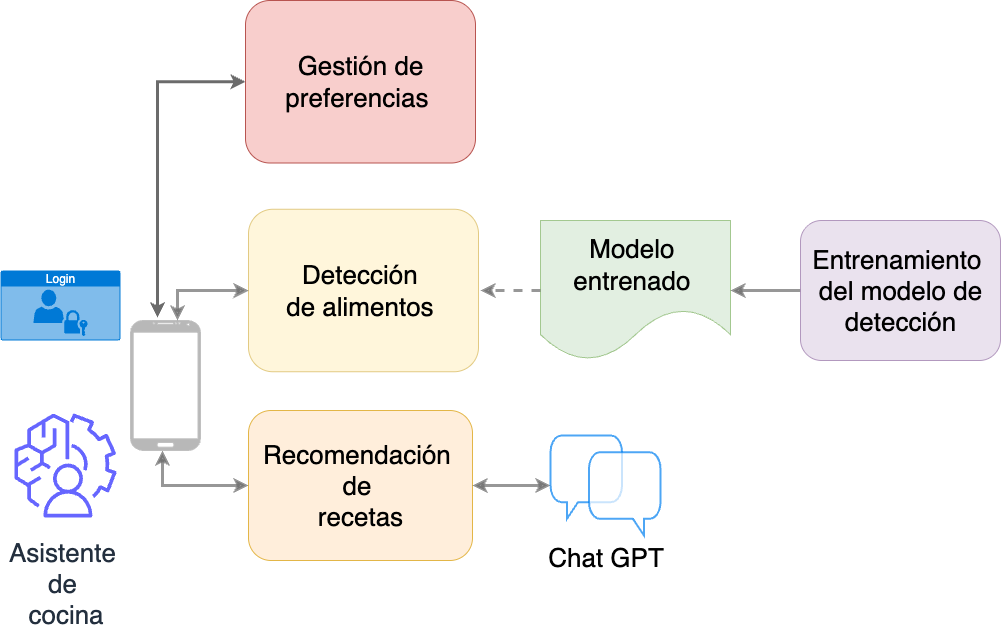
\includegraphics[width=.8\textwidth]{./Figuras/DiagramaGeneral.png}
\caption{Diagrama general de los módulos de la aplicación.}
\label{fig:DiagramaGeneral}
\end{figure}


La experiencia previa con el plan de proyectos de la CEIA ha proporcionado  una base sólida en la gestión de proyectos y se utilizó como bitácora de recursos para la confección de este plan.
\section{2. Identificación y análisis de los interesados}
\label{sec:interesados}

\begin{table}[H]
%\caption{Identificación de los interesados}
%\label{tab:interesados}
\begin{tabularx}{\linewidth}{@{}|l|X|X|l|@{}}
\hline
\rowcolor[HTML]{C0C0C0} 
Rol           & Nombre y Apellido & Organización 	& Puesto 	\\ \hline
Cliente       & \clientename      &\empclientename	& -       	\\ \hline
Responsable   & \authorname       & FIUBA        	& Alumno 	\\ \hline
Orientador    & \supname	      & \pertesupname 	& Director del Trabajo Final \\ \hline
Usuario final & Familiares y conocidos del responsable       & -             	&     -   	\\ \hline
\end{tabularx}
\end{table}


\begin{itemize}
	\item Responsable: el Ing. Fabricio Denardi es desarrollador desde hace más de 10 años y cursó la Carrera de Especialización en Inteligencia Artificial (CEIA) y la Maestría en Inteligencia Artificial (MIA), lo que le permitirá: elaborar los modelos de inteligancia artificial (IA) necesarios y el desarrollo de la aplicación junto con el despliegue de esta. Además, es un apasionado por la gastronomía.
	\item Orientador: el Dr. Ing. Facundo Lucianna es docente de la CEIA. Con su capacidad didáctica, colaborará con la definición de los requerimientos y aspectos técnicos, tanto de inteligencia artificial como los referidos al despliegue de la solución.
	\item Usuario final: si bien se espera que la aplicación a futuro tenga un fin comercial y sea vendida a tantos usuarios como sean posible, en un primer momento el responsable seleccionará familiares y conocidos que cumplan este rol, intentando ser lo más riguroso posible.
\end{itemize}


\section{3. Propósito del proyecto}
\label{sec:proposito}

Desarrollar un módulo de agente conversacional inteligente que extienda las funcionalidades de la aplicación previamente implementada para la detección de alimentos y recomendación de recetas. 

Con esta nueva funcionalidad se busca optimizar la experiencia de uso, incrementar la adaptabilidad del sistema frente a diferentes perfiles de usuarios y avanzar hacia una solución integral de apoyo culinario asistido por inteligencia artificial.

\section{4. Alcance del proyecto}
\label{sec:alcance}

El proyecto incluye:
\begin{itemize}
    \item Investigación y repaso de conceptos abordados en las diferentes materias, con especial énfasis en las asignaturas de Procesamiento del Lenguaje Natural I, II y III.
    \item Investigación y elaboración del presupuesto de los recursos necesarios para llevar a cabo el trabajo, tales como:
    \begin{itemize}
        \item Disponibilidad y costos de tokens de OpenAI.
        \item Uso de APIs externas (por ejemplo, APIs de Google u otras fuentes de información relevantes).
    \end{itemize}
    \item Desarrollo del asistente de cocina compuesto por diversos agentes:
    \begin{itemize}
        \item Subagente de recomendación:
        \begin{itemize}
            \item Generación y sugerencia de recetas.
            \item Consultas y sugerencias de cambios de ingredientes, variantes e instrucciones.
        \end{itemize}
        \item Agente de detección de objetos:
        \begin{itemize}
            \item Comunicación con el módulo de detección existente para recuperar los ingredientes a partir de la foto de los alimentos presentes en una heladera.
        \end{itemize}
        \item Agente de supermercado:
        \begin{itemize}
            \item Sugerencia de lugares donde adquirir los ingredientes faltantes.
        \end{itemize}
        \item Otros agentes:
        \begin{itemize}
            \item Si durante la construcción del trabajo se detectan funcionalidades adicionales de interés cuyo desarrollo no modifique significativamente el tiempo estimado de entrega, se evaluará su incorporación mediante el proceso de Gestión del Alcance.
        \end{itemize}
    \end{itemize}
    \item Incorporación de una interfaz gráfica en la aplicación móvil para la interacción con el agente.
    \item Elaboración de los manuales de arquitectura y de usuario.
    \item Redacción y presentación de la memoria final del trabajo.
\end{itemize}

\textbf{El presente proyecto no incluye:}
\begin{itemize}
    \item Implementación en producción de la solución.
    \item Implementación en entornos \textit{cloud}; el desarrollo se llevará a cabo exclusivamente en entornos locales.
    \item Modificaciones a los módulos existentes en la aplicación, tales como:
    \begin{itemize}
        \item Reentrenamiento del modelo YOLO de detección de objetos.
        \item Cambios en el módulo de recomendación.
        \item Modificaciones en la interfaz gráfica de las pantallas ya implementadas.
    \end{itemize}
\end{itemize}

\section{5. Supuestos del proyecto}
\label{sec:supuestos}
Para el proyecto se supone que:
\begin{itemize}
	\item El responsable contará con el tiempo extra laboral necesario para cumplir con todo el ciclo de vida del proyecto, entendiendo que el responsable del presente tiene sus obligaciones laborales y personales.
	\item Se dispondrá del dinero para licencias, equipos de entrenamiento y todos aquellos costos necesarios para el desarrollo de la aplicación.
	\item Se dispondrá de los accesos necesarios a todos los recursos y plataformas necesarios para el desarrollo del proyecto.
	\item En caso que el director/orientador no pueda colaborar en algunos aspectos técnicos referidos a visión por computadora, se conseguirá un co-director especialista en la temática.
	\item Se espera que los familiares y amigos del responsable que ofician como usuarios tendrán disponibilidad para realizar tareas de \textit{testing}.
\end{itemize}\section{6. Requerimientos}
\label{sec:requerimientos}

\begin{enumerate}
	\item Requerimientos funcionales:
	\begin{enumerate}
		\item Subagente de recomendación:
        \begin{enumerate}
            \item El agente debe generar y sugerir recetas basadas en los ingredientes disponibles.
            \item El agente debe permitir consultas sobre variantes de recetas y sustitución de ingredientes.
            \item El agente debe ofrecer sugerencias de modificaciones, alternativas o mejoras en las instrucciones de preparación.
        \end{enumerate}

        \item Subagente de detección de objetos:
        \begin{enumerate}
            \item El agente debe comunicarse con el módulo de detección existente para recuperar los ingredientes identificados en las imágenes.
            \item El agente debe procesar fotografías de alimentos tomadas desde una heladera u otro entorno similar.
            \item El agente debe devolver los ingredientes detectados en forma estructurada, listos para su uso por el subagente de recomendación.
        \end{enumerate}

        \item Subagente de supermercado:
        \begin{enumerate}
            \item El agente debe sugerir lugares o comercios donde adquirir los ingredientes faltantes.
            \item El agente debe consultar fuentes externas o APIs para ofrecer recomendaciones actualizadas de disponibilidad o ubicación.
        \end{enumerate}

		
       
    

		\item Aplicación para dispositivos celulares:
		\begin{enumerate}
			\item El usuario debe poder iniciar sesión en la aplicación.
			\item El usuario debe poder acceder al \textit{chat} con el agente a través de un acceso directo.
			\item El usuario debe poder realizar consultas al agente y recibir la respuesta de este.
		\end{enumerate}
	\end{enumerate}
	\item Requerimientos no funcionales:
		\begin{enumerate}
			\item Se debe poder contar con un repositorio en GitHub con todo el código fuente de todos los módulos.
			\item La aplicación para dispositivos celulares debe desarrollarse en Flutter.
			\item El resto de los módulos deben desarrollarse en Python.
			\item Los diferentes módulos deben estar organizados en \textit{docker containers}.
			\item De ser posible, se debe utilizar \textit{Apache Airflow} para la orquestación de los procesos.
		\end{enumerate}
	\item Requerimientos de documentación:
		\begin{enumerate}
			\item Se debe elaborar un diagrama a alto nivel con el diseño de la arquitectura del sistema.
			\item El usuario debe poder contar con un manual de usuario de la aplicación para dispositivos celulares.
		\end{enumerate}
	\item Requerimientos de testing:
		\begin{enumerate}
			\item El usuario final debe evaluar y certificar la aplicación a desarrollar.
		\end{enumerate}
	\item Requerimientos legales:
		\begin{enumerate}
			\item Siempre que sea posible, se debe utilizar herramientas de software libre para el desarrollo de los diferentes módulos. Se debe respetar las licencias que estos indiquen.
			\item Para el caso de componentes pagos, como por ejemplo Chat GPT, se tienen que utilizar de acuerdo al uso que se contrate.
			\item No se debe infringir ningún derecho de autor en las imágenes utilizadas para entrenar y verificar el modelo.
		\end{enumerate}
\end{enumerate}


\section{7. Historias de usuarios (\textit{Product backlog})}
\label{sec:backlog}

Para las historias de usuarios se identificaron los siguientes roles:
\begin{itemize}
\item Usuario: es la persona que utilizará la aplicación para dispositivos celulares.
\item Desarrollador: es la persona con conocimientos técnicos para desarrollar, mantener e implementar la solución completa. 
\end{itemize}


Para la ponderación de las historias de usuarios se utilizarán los siguientes criterios:

\begin{itemize}
\item Cantidad de trabajo: calificación de qué tanto trabajo (tiempo) implica la tarea.
\item Complejidad: dificultad técnica para llevar a cabo la tarea.
\item Incertidumbre: riesgo asociado a la tarea o cómo puede impactar en otras. 
\end{itemize}

\begin{table}[H]
%\caption{Ponderación de historias de usuario}
%\label{tab:ponderacionhistoriasusuario}
\begin{tabularx}{\linewidth}{@{}|l|X|X|l|@{}}
\hline
\rowcolor[HTML]{C0C0C0} 
	           & Cantidad de trabajo & Complejidad 	& Incertidumbre  \\ \hline
Baja       & 1     & 1	& 1      	\\ \hline
Media   & 3     & 3     	& 5 	\\ \hline
Alta    & 5      & 5 	& 8\\ \hline
\end{tabularx}
\end{table}


Cada historia tendrá un puntaje en cada categoría, se sumarán  y luego se buscará el número mayor o igual más próximo en la serie de Fibonacci.

\textbf{Historias de usuarios}\\
Historia de usuario 1 \\
Como usuario, quiero poder iniciar sesión en la aplicación para celulares (o buscarla en mi dispositivo) para poder almacenar mis preferencias y configuraciones.\\
Cantidad de trabajo: media. (3 puntos)\\
Complejidad: media. (3 puntos)\\
Incertidumbre: baja. (1 punto)\\
\textit{Story points:} 8 puntos.

Historia de usuario 2 \\
Como usuario, quiero poder tomar una foto en la aplicación para celulares (o buscarla en mi dispositivo) dentro del \textit{chat} con el agente para poder detectar los alimentos presentes en esta.\\
Cantidad de trabajo: media. (3 puntos)\\
Complejidad: media. (3 puntos)\\
Incertidumbre: baja. (1 punto)\\
\textit{Story points:} 8 puntos.

Historia de usuario 3 \\
Como usuario, quiero poder enviar la foto seleccionada al módulo de detección para recibir una lista de alimentos. \\
Cantidad de trabajo: alta. (5 puntos)\\
Complejidad: alta. (5 puntos)\\
Incertidumbre: alta. (8 puntos)\\
\textit{Story points:} 21 puntos.

Historia de usuario 4 \\
Como usuario, quiero poder enviar una lista de alimentos al agente para recibir una lista de recetas recomendadas. \\
Cantidad de trabajo: alta. (5 puntos)\\
Complejidad: alta. (5 puntos)\\
Incertidumbre: alta. (8 puntos)\\
\textit{Story points:} 21 puntos.

Historia de usuario 5 \\
Como usuario, quiero poder recibir del agente una lista de comercios donde puedo comprar los ingredientes faltantes. \\
Cantidad de trabajo: alta. (5 puntos)\\
Complejidad: alta. (5 puntos)\\
Incertidumbre: alta. (8 puntos)\\
\textit{Story points:} 21 puntos.

Historia de usuario 6 \\
Como usuario, quiero poder recibir del agente una lista de comercios para comprar los ingredientes faltantes de mi receta. \\
Cantidad de trabajo: alta. (5 puntos)\\
Complejidad: alta. (5 puntos)\\
Incertidumbre: alta. (8 puntos)\\
\textit{Story points:} 21 puntos.


Historia de usuario 7 \\
Como usuario, quiero poder recibir del agente recomendaciones de nutrición para adecuarme a las necesidades de mi dieta. \\
Cantidad de trabajo: alta. (5 puntos)\\
Complejidad: alta. (5 puntos)\\
Incertidumbre: alta. (8 puntos)\\
\textit{Story points:} 21 puntos.

Historia de usuario 8 \\
Como usuario, quiero poder recibir del agente una lista de ingredientes de reemplazo para cocinar de acuerdo a mis preferencias. \\
Cantidad de trabajo: media. (3 puntos)\\
Complejidad: media. (3 puntos)\\
Incertidumbre: baja. (1 punto)\\
\textit{Story points:} 8 puntos.

Historia de usuario 9 \\
Como usuario, quiero poder recibir del agente una lista de variantes de recetas para cocinar de acuerdo a mis preferencias. \\
Cantidad de trabajo: media. (3 puntos)\\
Complejidad: media. (3 puntos)\\
Incertidumbre: baja. (1 punto)\\
\textit{Story points:} 8 puntos.

Historia de usuario 10 \\
Como usuario, quiero poder recibir del agente recomendaciones sobre las instrucciones de las recetas devueltas por el módulo de recomendación para guiarme en la cocción del alimento. \\
Cantidad de trabajo: alta. (5 puntos)\\
Complejidad: alta. (5 puntos)\\
Incertidumbre: alta. (8 puntos)\\
\textit{Story points:} 21 puntos.

Historia de usuario 11 \\
Como usuario, quiero poder contar con un manual básico que muestre el uso de la aplicación para celulares.\\
Cantidad de trabajo: baja. (1 punto)\\
Complejidad: media. (1 punto)\\
Incertidumbre: baja. (1 punto)\\
\textit{Story points:} 3 puntos.

Historia de usuario 12 \\
Como desarrollador, quiero poder contar con un manual para consultar las métricas del modelo de detección.\\
Cantidad de trabajo: baja. (1 punto)\\
Complejidad: baja. (1 punto)\\
Incertidumbre: baja. (1 punto)\\
\textit{Story points:} 3 puntos.

Historia de usuario 13 \\
Como desarrollador, quiero poder contar con un documento técnico para consultar la arquitectura básica del sistema.\\
Cantidad de trabajo: baja. (1 punto)\\
Complejidad: baja. (1 punto)\\
Incertidumbre: baja. (1 punto)\\
\textit{Story points:} 3 puntos.

Historia de usuario 14 \\
Como usuario, quiero poder contar con un video o documento para visualizar un ejemplo \textit{end-to-end} del uso de la aplicación para celulares.\\
Cantidad de trabajo: baja. (1 punto)\\
Complejidad: baja. (1 punto)\\
Incertidumbre: baja. (1 punto)\\
\textit{Story points:} 3 puntos.


\section{8. Entregables principales del proyecto}
\label{sec:entregables}
Los entregables del proyecto serán:
\begin{itemize}
	\item Manual de usuario de la aplicación para celulares.
	\item Diagrama a alto nivel con el diseño de la arquitectura del sistema.
	\item Código fuente completo en un repositorio de \textit{GitHub}.
	\item Documento con las métricas obtenidas en el módulo del agente.
	\item Documento o video donde se muestre un ejemplo \textit{end-to-end} de la aplicación para celulares.
	\item Informes de avances.
	\item Memoria del trabajo final.
\end{itemize}


\section{9. Desglose del trabajo en tareas}
\label{sec:wbs}

\begin{enumerate}

\item Etapa de investigación. (56 h)
    \begin{enumerate}
        \item Investigar y repasar el material de la Maestría en Inteligencia Artificial sobre técnicas de modelos largos del lenguaje. (40 h)
        \item Evaluar y contratar la API de ChatGPT u otro LLM. (16 h)
    \end{enumerate}

\item Etapa de preprocesamiento y análisis exploratorio de los datos. (64 h)
    \begin{enumerate}
        \item Búsqueda de documentos de recetas de cocina. (40 h)
        \item Aplicar RAG sobre los documentos encontrados. (24 h)
    \end{enumerate}

\item Etapa de desarrollo del modelo del agente conversacional. (212 h)
    \begin{enumerate}
        \item Evaluar diferentes modelos que se adecuen al problema. (40 h)
        \item Desarrollar un subagente que se comunique con el módulo existente de detección de objetos. (24 h)
        \item Desarrollar un subagente que se comunique con el módulo existente de recomendación. (24 h)
        \item Desarrollar un subagente que se comunique con fuentes externas de localización de comercios. (40 h)
        \item Desarrollar un orquestador que gestione el pedido entre los distintos agentes y los otros módulos. (80 h)
        \item Pruebas unitarias y de integración de la API propia. (4 h)
    \end{enumerate}

\item Etapa de desarrollo de la aplicación para celulares. (128 h)
    \begin{enumerate}
        \item Armar la estructura general del chat. (40 h)
        \item Agregar interfaz de comunicación con el módulo del agente. (24 h)
        \item Agregar funcionalidades de interacción entre el usuario y el chat. (40 h)
        \item Armar pantalla de login. (24 h)
    \end{enumerate}

\item Etapa de \textit{User Acceptance Testing (UAT)}. (36 h)
    \begin{enumerate}
        \item Ciclo de pruebas 1 de la aplicación para celulares. (16 h)
        \item Correcciones de los defectos o errores detectados en el ciclo de pruebas 1. (8 h)
        \item Ciclo de pruebas 2 de la aplicación para celulares. (8 h)
        \item Correcciones de los defectos o errores detectados en el ciclo de pruebas 2. (4 h)
    \end{enumerate}

\item  Etapa de documentación. (56 h)
    \begin{enumerate}
        \item Elaboración del manual de usuario para la aplicación para celulares. (24 h)
        \item Elaboración del documento de arquitectura a alto nivel. (8 h)
        \item Elaboración de reporte de métricas del modelo de detección de objeto. (8 h)
        \item Elaboración de video o documento con ejemplo de funcionamiento de la aplicación para celular. (16 h)
    \end{enumerate}

\item Etapa de cierre. (57 h)
    \begin{enumerate}
        \item Redacción de informes de avance. (8 h)
        \item Redacción de la memoria final. (40 h)
        \item Elaboración y preparación de la presentación final. (8 h)
        \item Defensa del trabajo final. (1 h)
    \end{enumerate}

\end{enumerate}

Cantidad total de horas: 609 h.


\section{10. Diagrama de Activity On Node}
\label{sec:AoN}
A continuación, se realiza una breve descripción del diagrama \textit{Activity on Node}:

\begin{itemize}
\item La duración de las tareas (t) está expresada en horas.
\item Las tareas de la etapa de preprocesamiento y análisis exploratorio de los datos pueden realizarse en paralelo.
\item El desarrollo de los módulos de detección de objetos y predicción de recetas pueden realizarse en paralelo.
\item El desarrollo de la aplicación para celulares debe comenzar una vez que hayan sido finalizados los módulos de detección de objetos y predicción de recetas.
\item El camino crítico está marcado en rojo y su duración es de 593 horas.
\end{itemize}


\begin{figure}[htpb]
\centering 
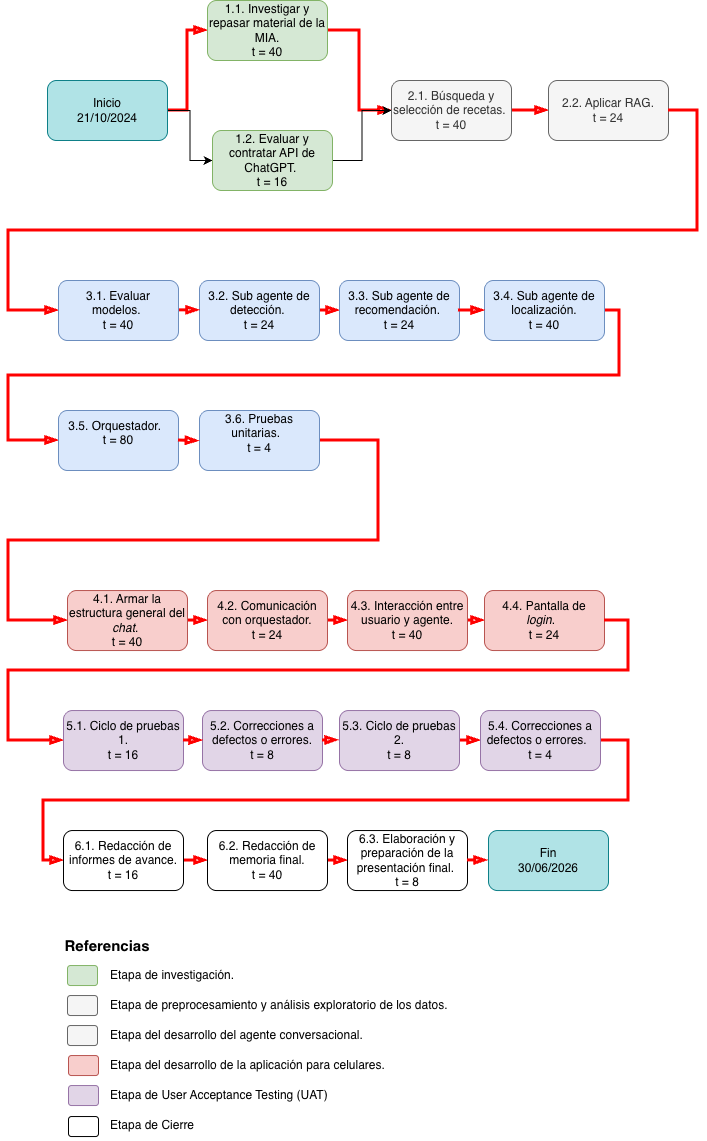
\includegraphics[width=.8\textwidth]{./Figuras/AoN-MIA.png}
\caption{Diagrama de \textit{Activity on Node}.}
\label{fig:AoN}
\end{figure}



\section{11. Diagrama de Gantt}
\label{sec:gantt}

\begin{figure}[H]
\centering 
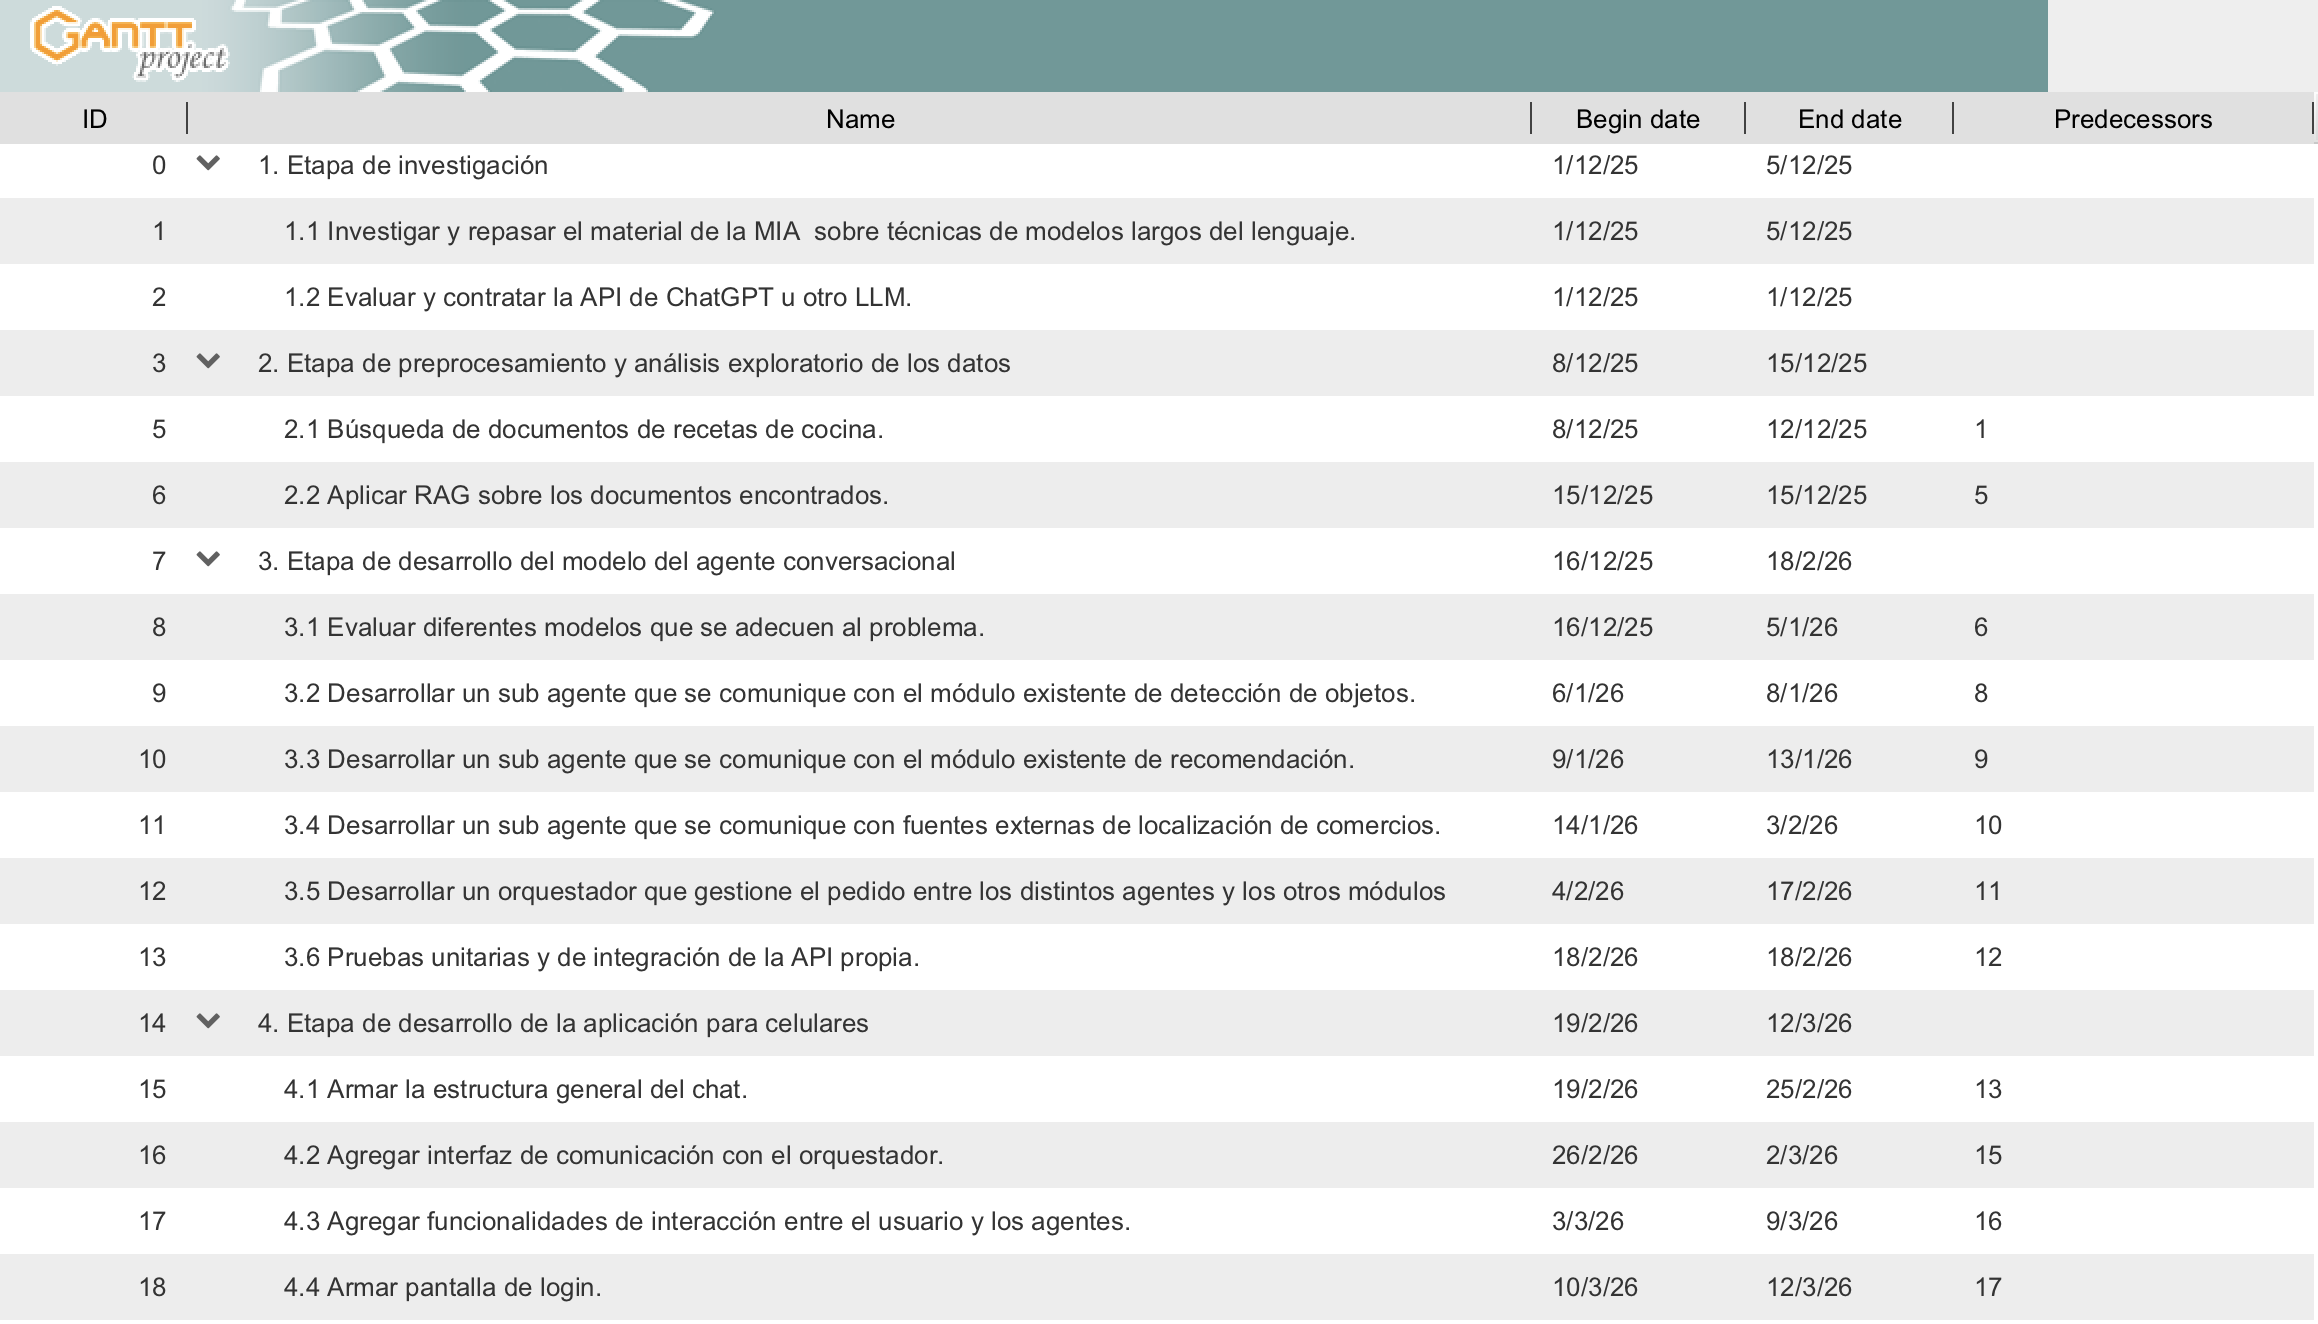
\includegraphics[width=1\textwidth]{./Figuras/gantt_1_1.png}\\[0.5em]
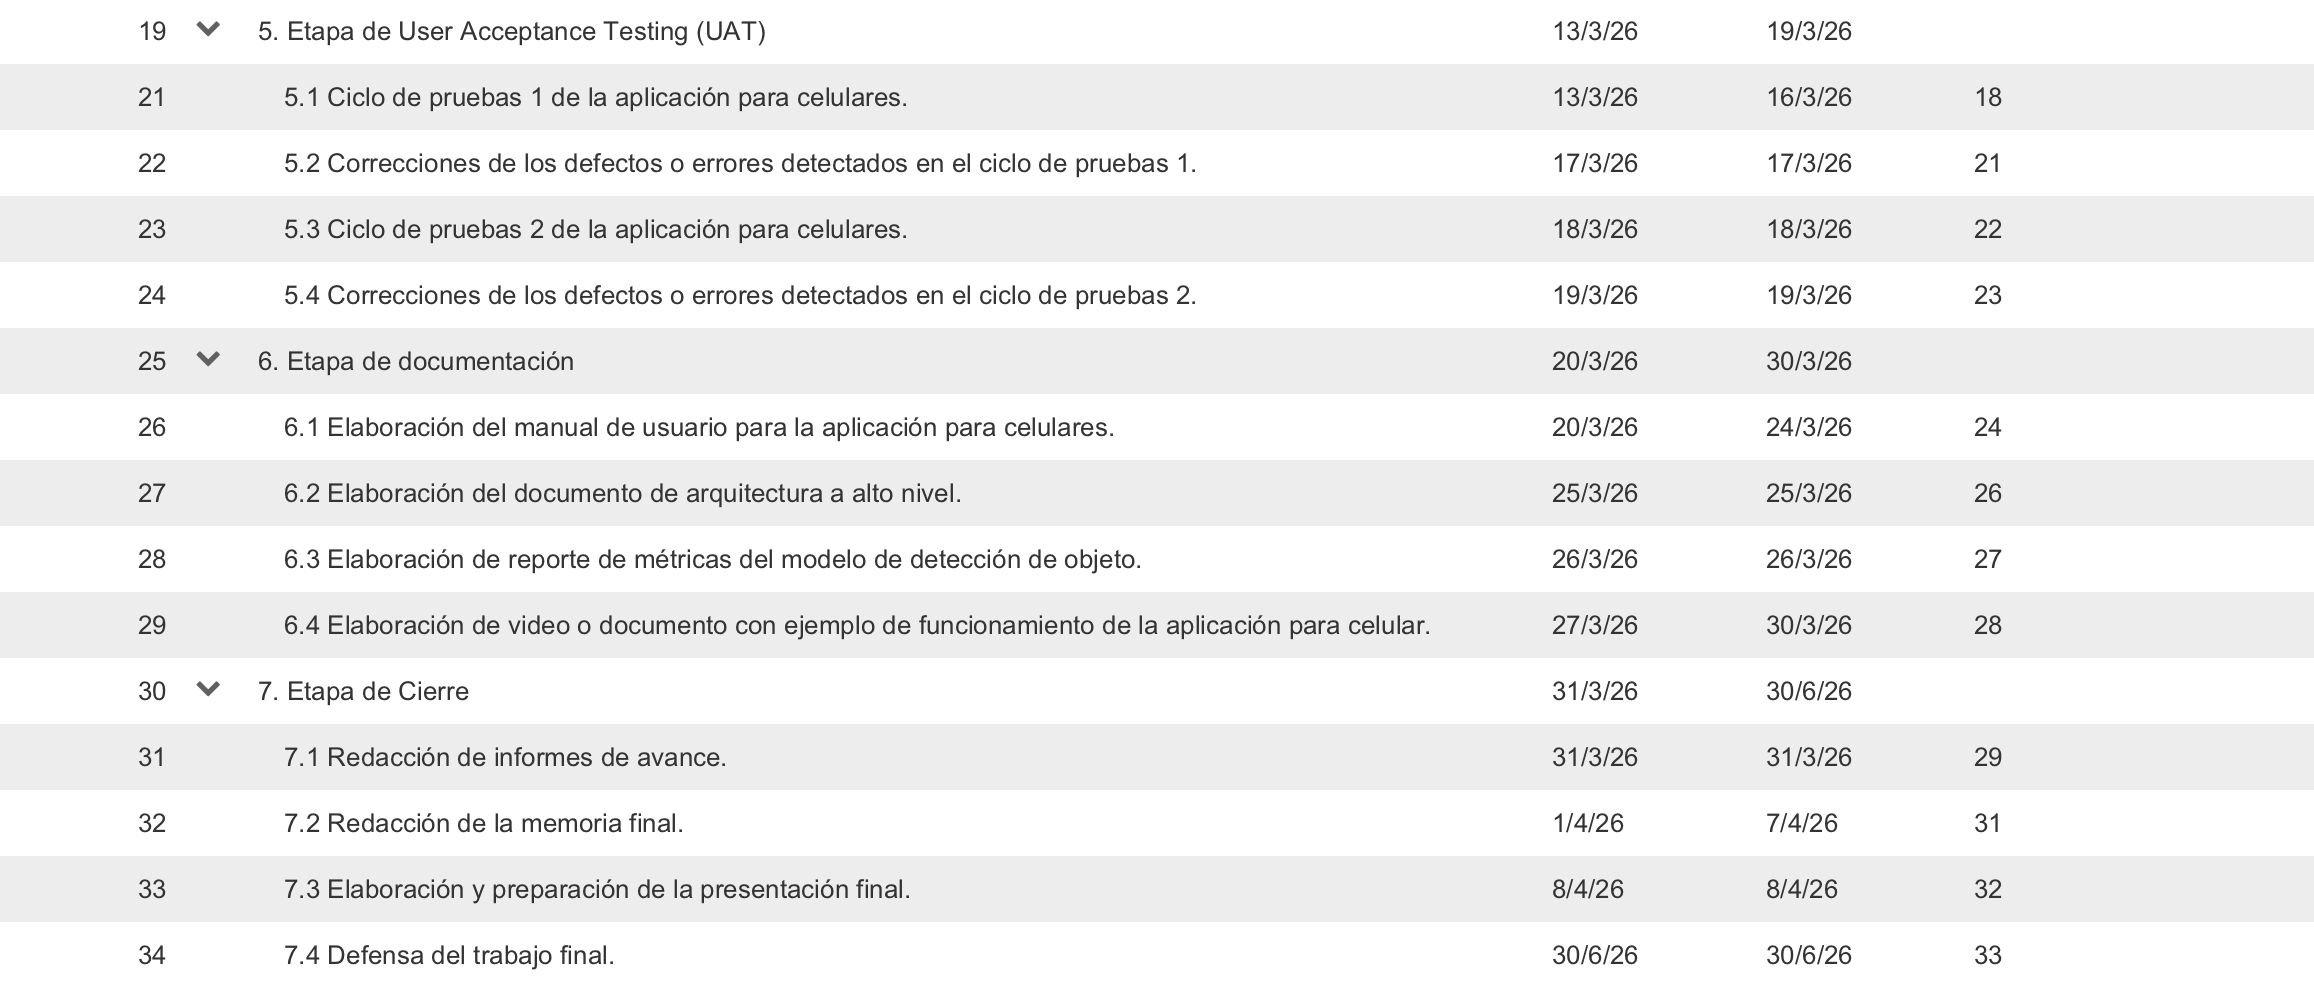
\includegraphics[width=1\textwidth]{./Figuras/gantt_1_2.png}
\caption{EDT.}
\label{fig:AoN}
\end{figure}

\newpage
\begin{landscape}
\begin{figure}[H]
\centering 
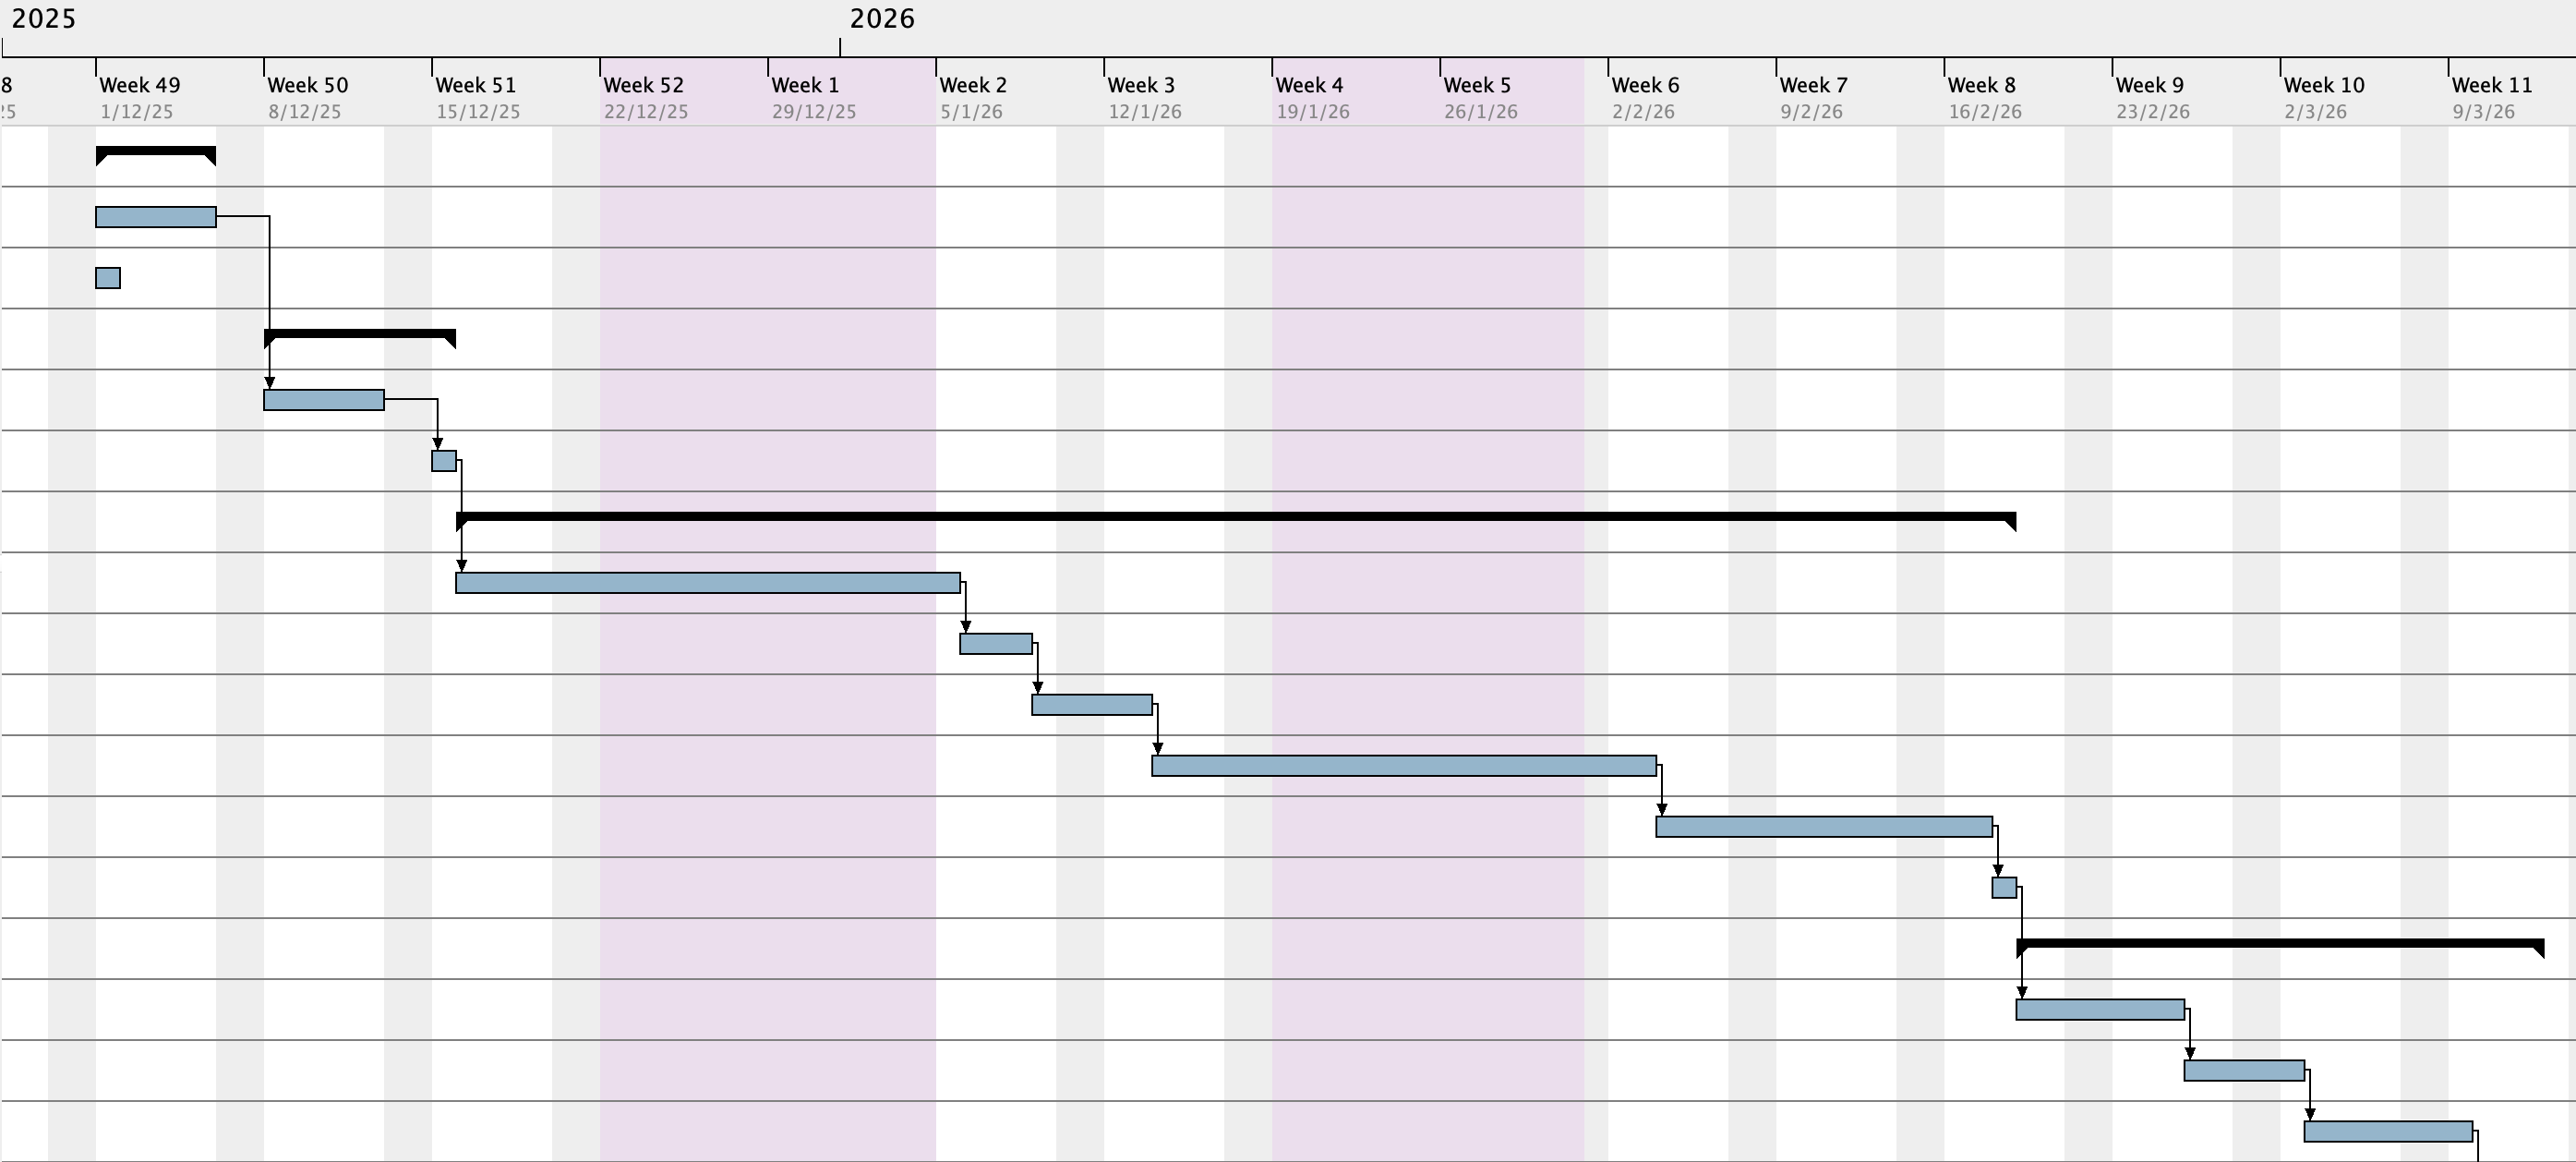
\includegraphics[width=1.55\textwidth]{./Figuras/gantt_2_1.png}
\label{fig:Gantt 2.1}
\end{figure}
\end{landscape}

\begin{landscape}
\begin{figure}[H]
\centering 
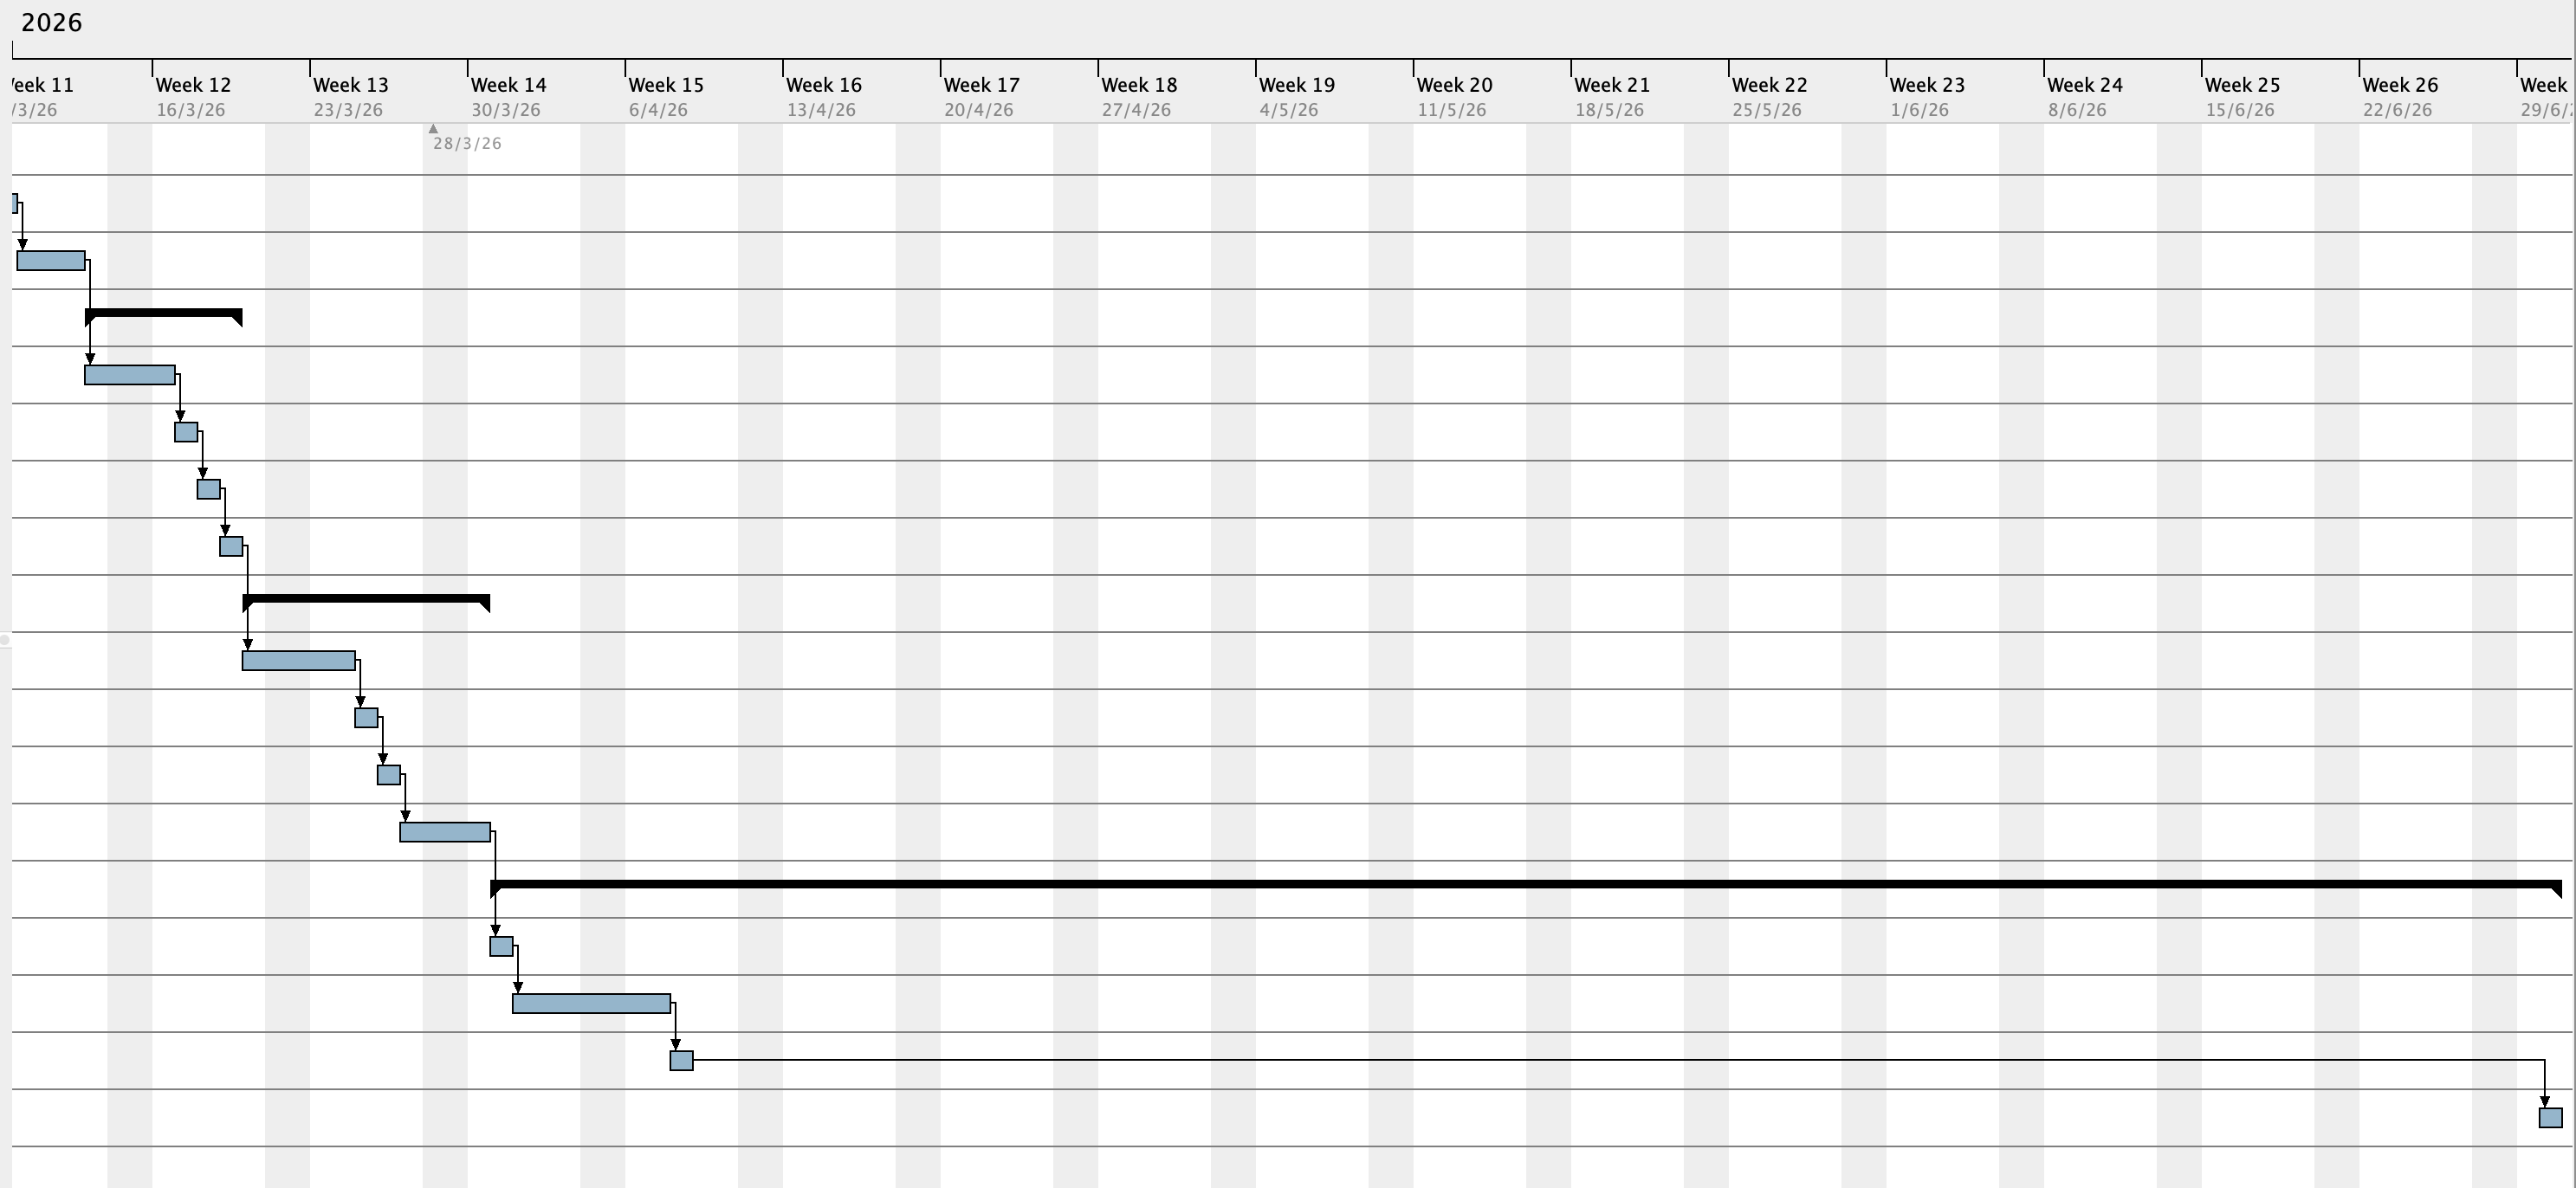
\includegraphics[width=1.5\textwidth]{./Figuras/gantt_2_2.png}
\caption{Gantt}
\label{fig:Gantt 2.2}
\end{figure}
\end{landscape}


\section{12. Presupuesto detallado del proyecto}
\label{sec:presupuesto}

\begin{table}[htpb]
\centering
\begin{tabularx}{\linewidth}{@{}|X|c|r|r|@{}}
\hline
\rowcolor[HTML]{C0C0C0} 
\multicolumn{4}{|c|}{\cellcolor[HTML]{C0C0C0}COSTOS DIRECTOS} \\ \hline
\rowcolor[HTML]{C0C0C0} 
Descripción &
  \multicolumn{1}{c|}{\cellcolor[HTML]{C0C0C0}Cantidad} &
  \multicolumn{1}{c|}{\cellcolor[HTML]{C0C0C0}Valor unitario} &
  \multicolumn{1}{c|}{\cellcolor[HTML]{C0C0C0}Valor total} \\ \hline
 
  Horas de ingeniería del responsable. &
  \multicolumn{1}{c|}{600} &
  \multicolumn{1}{c|}{ARS 180.000,00 } &
  \multicolumn{1}{c|}{ARS 108.000.000,00} \\ \hline

  
  Licencia Chat GPT Plus (USD 20,00). &
  \multicolumn{1}{c|}{6} &
  \multicolumn{1}{c|}{ARS 28.800,00} &
  \multicolumn{1}{c|}{ARS 172.800,00} \\ \hline
  
  
\multicolumn{1}{|l|}{} &
   &
   &
   \\ \hline
\multicolumn{1}{|l|}{} &
   &
   &
   \\ \hline
\multicolumn{3}{|c|}{SUBTOTAL} &
  \multicolumn{1}{c|}{ARS 108.172.800,00} \\ \hline
\rowcolor[HTML]{C0C0C0} 
\multicolumn{4}{|c|}{\cellcolor[HTML]{C0C0C0}COSTOS INDIRECTOS} \\ \hline
\rowcolor[HTML]{C0C0C0} 
Descripción &
  \multicolumn{1}{c|}{\cellcolor[HTML]{C0C0C0}Cantidad} &
  \multicolumn{1}{c|}{\cellcolor[HTML]{C0C0C0}Valor unitario} &
  \multicolumn{1}{c|}{\cellcolor[HTML]{C0C0C0}Valor total} \\ \hline
\multicolumn{1}{|l|}{20	\% de los costos directos.} & 1
   & ARS 21.634.560,00
   & ARS 21.634.560,00
   \\ \hline
\multicolumn{1}{|l|}{} &
   &
   &
   \\ \hline
\multicolumn{1}{|l|}{} &
   &
   &
   \\ \hline
\multicolumn{3}{|c|}{SUBTOTAL} &
  \multicolumn{1}{c|}{ARS 10.885.362} \\ \hline
\rowcolor[HTML]{C0C0C0}
\multicolumn{3}{|c|}{TOTAL} & ARS 129.807.360,00
   \\ \hline
\end{tabularx}%
\end{table}

Nota: la tasa de cambio  utilizada fue la del Banco de la Nación Argentina (BNA), tipo vendedor, al 16 de octubre de 2025 (USD 1 = ARS 1.440,00). 


\section{13. Gestión de riesgos}
\label{sec:riesgos}
Se han identificado los siguientes riesgos: 

Riesgo 1: no contar con suficientes imágenes de calidad para entrenar el modelo de detección de objetos.
\begin{itemize}
\item Severidad (S): tener una buena calidad de imágenes es crucial para un buen entrenamiento de modelos de inteligencia artificial. Sin datos de calidad, las métricas de cualquier modelo son extremadamente pobres. (10)
\item Probabilidad de ocurrencia (O): con frecuencia los datasets disponibles en los sitios web son limitados en cuanto a la cantidad y calidad de imágenes. Adicionalmente, suelen tener poco ruido o diversidad, lo que los alejan de las imágenes reales que un usuario de la aplicación utilizará en la inferencia. (9)
\end{itemize}

Riesgo 2: falta de conocimientos técnicos para la realización del modelo de detección de objetos.
\begin{itemize}
\item Severidad (S): contar con conocimientos técnicos en modelos de visión por computadoras es fundamental para lograr métricas eficientes y eficaces. (7)
\item Probabilidad de ocurrencia (O):  el responsable ya cuenta con una base en la temática dado que cursó dos materias en la CEIA, sin embargo pueden no ser suficientes. (7)
\end{itemize}

Riesgo 3: no contar con dinero suficiente para afrontar el presupuesto del proyecto.
\begin{itemize}
\item Severidad (S): sin los recursos adecuados no se puede realizar el entrenamiento del módulo de detección de objetos y no será posible realizar la inferencia utilizando las API de Chat GPT. Existen recursos gratuitos que podrían soportar los requerimientos parcialmente. (9)
\item Probabilidad de ocurrencia (O): el responsable ya evaluó los costos que deberá incurrir y tiene el dinero ahorrado disponible para afrontarlos. (2)
\end{itemize}

Riesgo 4: no cumplir con los tiempos de finalización del proyecto.
\begin{itemize}
\item Severidad (S): el responsable tiene pensado continuar con la especialización en internet de las cosas, con lo que un atraso en el trabajo final conllevaría a un atraso en el comienzo de la nueva especialización. Dado que no tiene dedicación exclusiva, no puede hacer las dos cosas a la vez. La severidad no es tan alta ya que FIUBA abre cohortes de todas las especializaciones varias veces al año. (2)
\item Probabilidad de ocurrencia (O): el responsable trabaja \textit{fulltime} y se encuentra con proyectos importantes en la compañía para la que trabaja, requiriéndole horas extras para cumplir. (10)
\end{itemize}

Riesgo 5: no conseguir suficientes amigos y familiares que oficien como usuarios finales.
\begin{itemize}
\item Severidad (S): sin un buen \textit{testing} es probable que la calidad del producto final no sea la esperada. El responsable tiene conocimientos gastronómicos con lo que algunas pruebas podría hacerlas el mismo. La gastronomía no es una ciencia que requiere elevado conocimiento específico. (5)
\item Probabilidad de ocurrencia (O): muchos familiares y amigos ya se han comprometido de palabra con el responsable para realizar estas tareas. (2)
\end{itemize}



\begin{table}[htpb]
\centering
\begin{tabularx}{\linewidth}{@{}|X|c|c|c|c|c|c|@{}}
\hline
\rowcolor[HTML]{C0C0C0} 
Riesgo & S & O & RPN & S* & O* & RPN* \\ \hline
Riesgo 1: no contar con suficientes documentos de recetas para construir la base de datos vectoriales y el RAG.      & 10   & 8  &  80   & 10   &  1  &   10   \\ \hline
Riesgo 2: falta de conocimientos técnicos para la realización del modelo de detección de objetos.     & 7  & 7  &  49   & 7   &  2  &    14  \\ \hline
Riesgo 3: no contar con dinero suficiente para afrontar el presupuesto del proyecto.       & 9  & 2  &   18  &    &    &      \\ \hline
Riesgo 4: no cumplir con los tiempos de finalización del proyecto.       &  2 & 10  &   20  &    &    &      \\ \hline
Riesgo 5: no conseguir suficientes amigos y familiares que oficien como usuarios finales.       & 5  &  2 &    10 &    &    &      \\ \hline
\end{tabularx}%
\end{table}

Criterio adoptado: se tomarán medidas de mitigación en los riesgos cuyos números de RPN
sean mayores a 45.

Nota: los valores marcados con (*) en la tabla corresponden luego de haber aplicado la
mitigación del riesgo.


\textbf{Plan de mitigación de los riesgos que originalmente excedan el RPN máximo establecido}\\\\
Riesgo 1: solicitar colaboración a instituciones educativas de gastronomía para que provean recetas modelos, a cambio de publicidad en la aplicación.

Nueva asignación de S y O, con su respectiva justificación:
\begin{itemize}
\item Severidad (S): la severidad no cambia ya que malos datos seguirán generando malos modelos. (10)
\item Probabilidad de ocurrencia (O): la probabilidad de ocurrencia cae drásticamente ya que son imágenes que se pueden conseguir fácilmente por cualquier persona (solamente usando su dispositivo celular). (1)
\end{itemize}

Riesgo 2: conseguir un codirector con conocimientos en modelos largos del lenguaje y solicitar ayuda a graduados y colegas de la CEIA o la MIA.

Nueva asignación de S y O, con su respectiva justificación:
\begin{itemize}
\item Severidad (S):  si aun con la ayuda de un codirector o colegas no se logra reforzar los conocimientos técnicos, la \textit{performance} del modelo será baja y no logrará buenas detecciones de alimentos. (7)
\item Probabilidad de ocurrencia (O): con la ayuda de varios especialistas en este tipo de modelos es poco probable llegar a malos modelos de detección. (2)
\end{itemize}


\section{14. Gestión de la calidad}
\label{sec:calidad}

\begin{consigna}{red}
Elija al menos diez requerimientos que a su criterio sean los más importantes/críticos/que aportan más valor y para cada uno de ellos indique las acciones de verificación y validación que permitan asegurar su cumplimiento.

\begin{itemize} 
\item Req \#1: copiar acá el requerimiento con su correspondiente número.

\begin{itemize}
	\item Verificación para confirmar si se cumplió con lo requerido antes de mostrar el sistema al cliente. Detallar.
	\item Validación con el cliente para confirmar que está de acuerdo en que se cumplió con lo requerido. Detallar. 
\end{itemize}

\end{itemize}

Tener en cuenta que en este contexto se pueden mencionar simulaciones, cálculos, revisión de hojas de datos, consulta con expertos, mediciones, etc.  

Las acciones de verificación suelen considerar al entregable como ``caja blanca'', es decir se conoce en profundidad su funcionamiento interno.  

En cambio, las acciones de validación suelen considerar al entregable como ``caja negra'', es decir, que no se conocen los detalles de su funcionamiento interno.

\end{consigna}

\section{15. Procesos de cierre}    
\label{sec:cierre}


\begin{itemize}
	\item Pautas de trabajo que se seguirán para analizar si se respetó el Plan de Proyecto original:
	 \begin{itemize}
	 \item Responsable: Ing. Fabricio Denardi.
	 \item Procedimiento:
	 \begin{enumerate}
	 	\item Revisar el proyecto original y sus objetivos.
	 	\item Comprobar los entregables realizados con los planificados en el plan original.
	 	\item Evaluar los recursos utilizados respecto a los planificados.
	 	\item Identificar cambios y desvíos en el alcance, tiempo y presupuesto.
	 	\item Documentar los cambios y desvíos en caso que los haya habido. 	
	 \end{enumerate}
	 \end{itemize}
	\item Identificación de las técnicas y procedimientos útiles e inútiles que se emplearon, los problemas que surgieron y cómo se solucionaron:
	\begin{itemize}
	 \item Responsable: Ing. Fabricio Denardi.
	 \item Procedimiento:
	 \begin{enumerate}
	 	\item Revisar las técnicas y procedimientos que se utilizaron en el proyecto.
	 	\item Identificar aquellas que han sido efectivas y contribuyeron al éxito del proyecto.
	 	\item Identificar las que, por el contrario, resultaron ineficaces y causaron problemas.
	 	\item Realizar una videollamada con el director del trabajo final en donde se discutan estas técnicas y procedimiento. Adicionalmente, en esta videollamada se deben establecer las lecciones aprendidas que dejó este proyecto.
	 	\item Elaborar un informe de las lecciones aprendidas discutidas en la videollamada.
	 \end{enumerate}
	 
	 \end{itemize}
	\item Indicar quién organizará el acto de agradecimiento a todos los interesados, y en especial, al equipo de trabajo y colaboradores:
	 \begin{itemize}
	 \item Responsable: Ing. Fabricio Denardi.
	 \item Procedimiento:
	 \begin{enumerate}
	 	\item Organizar un acto de agradecimiento en donde participen todos los interesados. Este acto se debe hacer mediante una videoconferencia.
	 \end{enumerate}
	 
	 \end{itemize}
	 
	 \item Realizar una presentación y demostración pública del proyecto ante los jurados. 
	  \begin{itemize}
	 \item Responsable: Ing. Fabricio Denardi.
	 \item Procedimiento:
	 \begin{enumerate}
	 \item El responsable debe coordinar con la FIUBA la presentación y demostración pública.
	 	\item El responsable debe presentar su proyecto ante los jurados y el público en general.
	 \end{enumerate}
	 \end{itemize}
\end{itemize}

\end{document}